\documentclass[../presentation.tex]{subfiles}

\begin{document}

% \section{Example - Double Gyre}
\begin{frame}
  \frametitle{Validation - Double Gyre}
  
  \begin{itemize}
    \item Let's look at the double gyre flow. This flow comes from hamiltonian stream function.
    \begin{equation}
      \begin{aligned}
        \Psi(x, y, t) &= A\sin(\pi f(x, t)) \sin(\pi y)
      \end{aligned}
    \end{equation}
    
    \item Where,
    \begin{equation}
      \begin{aligned}
        f(x, t) = \epsilon\sin(wt) x^2 + (1 - 2 \epsilon \sin(wt))x
      \end{aligned}
    \end{equation}
%   \end{itemize}
% \end{frame}

% \begin{frame}
%   \frametitle{Validation - Double Gyre}

%   \begin{itemize}
    \item We can calculate the velocity field \(V = (U, V)\) as
    \begin{itemize}
      \item\begin{equation}
        \begin{aligned}
          \dot x &= U(x, y, t) \\
          &= -A\pi\sin(\pi f(x, t)) cos(\pi y) \\
        \end{aligned}
      \end{equation}
      
      \item \begin{equation}
        \begin{aligned}
          \dot y &= v(x, y, t) \\
          &= A\pi\cos(\pi f(x, t)) \sin(\pi y) \frac{\partial F}{\partial x}
        \end{aligned}
      \end{equation}
    \end{itemize}
  \end{itemize}  
\end{frame}

\begin{frame}
  \frametitle{Validation - Double Gyre}
  \begin{figure}
    \centering
    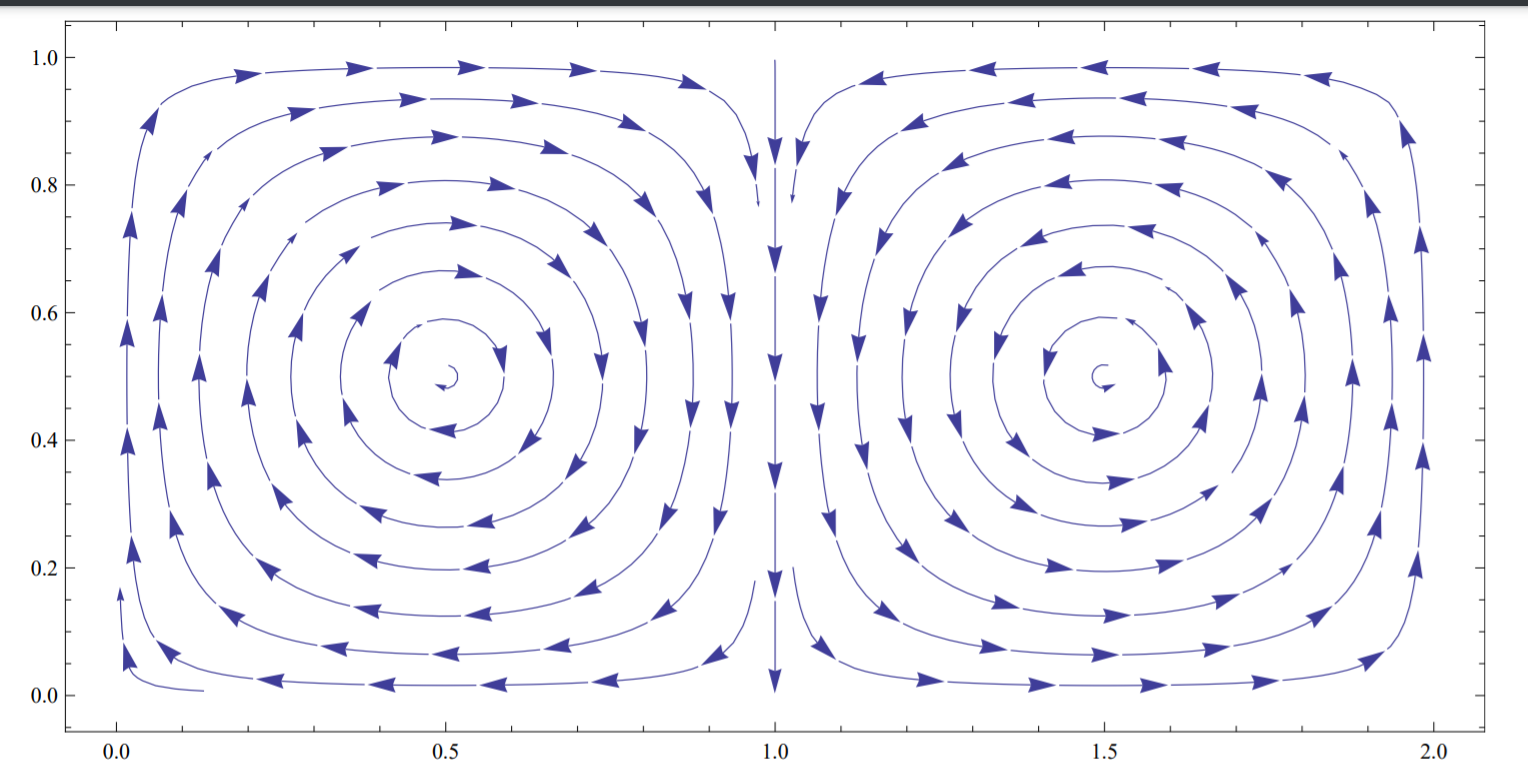
\includegraphics[width=\linewidth]{images/image_2.png}
    \caption{Streamline flow of Double Gyre}
    \label{figg:fig_2}
  \end{figure}
\end{frame}

\begin{frame}
  \frametitle{Validation - Double Gyre}

  \begin{itemize}
    \item We use the parameters, \(A = 0.1\), \(w = 0.2\pi\) and \(\epsilon = 0.25\)
  \end{itemize}
  
  {\tiny
    \begin{equation}
      \begin{aligned}
        \therefore \nabla V &= \begin{bmatrix}
          \frac{\partial U}{\partial x} & \frac{\partial U}{\partial y} \\[12pt]
          \frac{\partial V}{\partial x} & \frac{\partial V}{\partial y} \\
        \end{bmatrix} \\
        &= \begin{bmatrix}
          -\pi^2 A\cos(\pi f)\cos(\pi y) \frac{\partial f}{\partial x} & \pi^2 A\sin(\pi f)\sin(\pi y) \\[12pt]
          -\pi^2 A\sin(\pi f)\sin(\pi y)\frac{\partial f}{\partial x} + \pi A\cos(\pi f)\sin(\pi y) \frac{\partial^2 f}{\partial x^2} & \pi^2 A\cos(\pi f)\cos(\pi y)\frac{\partial f}{\partial x} \\
        \end{bmatrix}
      \end{aligned}
    \end{equation}
  }

  \begin{itemize}
    \item Now Eulerian Rate of Strain Tensor,
  \end{itemize}
  \begin{equation}
    \begin{aligned}
      \therefore \nabla V &= \begin{bmatrix}
        \frac{\partial U}{\partial x} & \frac{1}{2} (\frac{\partial U}{\partial y} + \frac{\partial V}{\partial x}) \\[12pt]
        \frac{1}{2} (\frac{\partial U}{\partial y} + \frac{\partial V}{\partial x}) & \frac{\partial V}{\partial y} \\
      \end{bmatrix} \\
    \end{aligned}
  \end{equation}
\end{frame}

\begin{frame}
  \frametitle{Validation - Double Gyre}

  \begin{figure}[H]
    \centering
    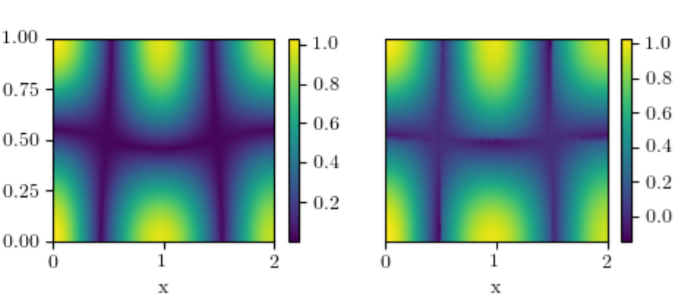
\includegraphics[width=\linewidth]{images/figure6.png}
  \end{figure}
\end{frame}

\begin{frame}
  \frametitle{Validation - Double Gyre}

  \begin{itemize}
    \item Now the below figure shows a comparison of the FTLE field for a short integration Time \(T = -0.5\) first with an approximation to first order in \(T\).
  \end{itemize}

  \begin{figure}[H]
    \centering
    \begin{minipage}{.5\textwidth}
        \centering
        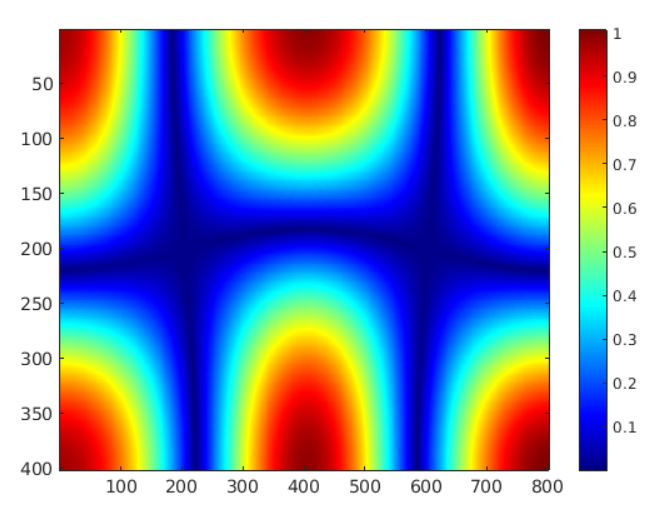
\includegraphics[width=\linewidth]{images/figure7.png}
    \end{minipage}%
    \begin{minipage}{0.5\textwidth}
        \centering
        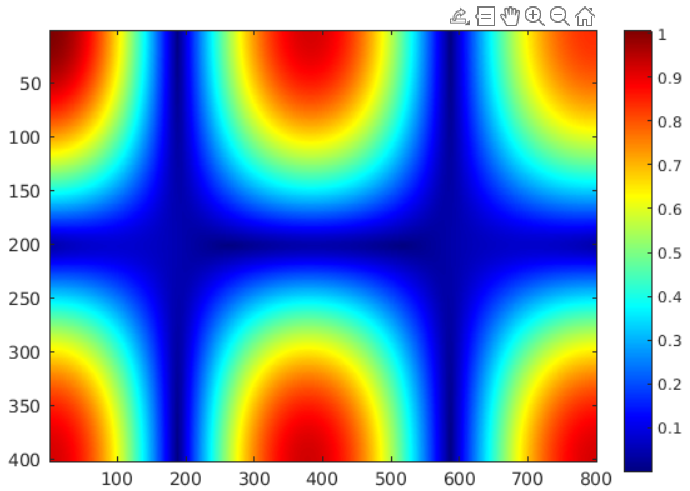
\includegraphics[width=\linewidth]{images/figure8.png}
    \end{minipage}
    % \caption{\tiny Left: FTLE field for the double-gyre flow for an integration period of T = -0.3. Right: approximation to the FTLE field to first-order in T. Parameters: A = 0.1, w = 0.2 e = 0.25, and to = 0.}
    \label{fig:fig_3}
  \end{figure}
\end{frame}



\end{document}